\documentclass[conference]{IEEEtran}
\IEEEoverridecommandlockouts
% The preceding line is only needed to identify funding in the first footnote. If that is unneeded, please comment it out.
\usepackage{cite}
\usepackage{amsmath,amssymb,amsfonts}
\usepackage{algorithmic}
\usepackage{graphicx}
\usepackage{textcomp}
\usepackage{xcolor}
\def\BibTeX{{\rm B\kern-.05em{\sc i\kern-.025em b}\kern-.08em
    T\kern-.1667em\lower.7ex\hbox{E}\kern-.125emX}}
\begin{document}

\title{Dynamic Load Balancing for Particle-in-Cell, CFD, and Discrete Event Simulations\\
\thanks{Identify applicable funding agency here. If none, delete this.}
}

\author{\IEEEauthorblockN{1\textsuperscript{st} Gerrett Diamond}
\IEEEauthorblockA{\textit{SCOREC} \\
\textit{Rensselaer Polytechnic Institute}\\
Troy, NY\\
diamog@rpi.edu}
\and
\IEEEauthorblockN{2\textsuperscript{nd} Cameron W. Smith}
\IEEEauthorblockA{\textit{SCOREC} \\
\textit{Rensselaer Polytechnic Institute}\\
Troy, NY\\
smithc11@rpi.edu}
\and
\IEEEauthorblockN{3\textsuperscript{rd} Mark S. Shephard}
\IEEEauthorblockA{\textit{SCOREC} \\
\textit{Rensselaer Polytechnic Institute}\\
Troy, NY\\
shephard@rpi.edu}
}

\maketitle

\begin{abstract}

\end{abstract}

\begin{IEEEkeywords}
component, formatting, style, styling, insert
\end{IEEEkeywords}

\section{Introduction}

\begin{itemize}
\item motivate dynamic load balancing
\item talk about how different applications have different partitioning needs
\item Mention that engpar is general to support a range of structures.
\end{itemize}

\section{EnGPar}

\begin{itemize}
\item Discuss the Ngraph in general graph terms with some figures
\item Discuss dynamic load balancing and the general diffusive steps
\end{itemize}

\section{Particle In Cell}

\begin{itemize}
\item Briefly discuss PIC/XGCM
\item Mention that the mesh partition is static.
\item Describe the buffer/safe zone
\item Describe the weight diffusion algorithm.
\end{itemize}

Since the mesh partitions in XGCM are fixed based on the geometry, we only consider
load balancing the particles. The main consideration when migrating particles in XGCM
is that a particle must always be in an element that is in the safe zone of a part.
This means that if a particle moves outside the safe zone, it must be migrated to a
new process where it is safe and when load balancing particles we must ensure that every
particle is migrated to a process where it is in the safe zone of the part.

To handle both cases, we construct the N-graph carefully such that any partition
decision in EnGPar will always maintain this requirement in XGCM. First we define
the components of XGCM by the following: {\color{red} Probably should turn these lists
  into full text instead.}
\begin{itemize}
\item Let $F = \{F_1,F_2, ..., F_n\}$ be the flux faces.
\item Let $G = \{G_1, G_2, ..., G_n\}$ be the groups such that $G_i$
  contains $F_i$ and the suitable buffer region around $F_i$
\item Let $S = \{S_1,S_2,...,S_n\}$ be the safe zones for each $G_i$.
  It is required that $S_i \subset G_i$.
\item Define $\bar{S_j}$ for each set of overlapping safe zones.
\item Let $P$ be the set of particles.
\item For each particle $p\in P$, Let $T_p$ be the set of safe zones in $S$ that $p$ resides
  in.  $\forall p \in P, \exists ! i$ such that $T_p = \bar{S_i}$.
\item  Let $P_{\bar{S_i}}$ be the set of particles such that $\forall p \in P_{\bar{S_i}}, T_p = \bar{S_i}$.
\end{itemize}

With these definitions, we define the Ngraph as $G = \{V, H, P\}$ where:
\begin{enumerate}
\item $V = \{ v_{i,j}$ for each $\bar{S_i} | S_j \in \bar{S_i} \}$.
\item The weight of vertex $v_{t,i}$ is equal to $|P_{\bar{S_i}}|$ on process $t$.
\item $H = \{ h_i$ for each $\bar{S_i} \}$.
\item $P = \{ p_{i,j}$ connecting $v_{i,j}$ to $h_i \}$.
\end{enumerate}
Figure \ref{fig:sbars} shows an example of the $\bar{S_i}$ and the construction of N-graph from
them. {\color{red} Make example figure smaller so it is visible in paper.}

\begin{figure}[!ht]
  \centering
  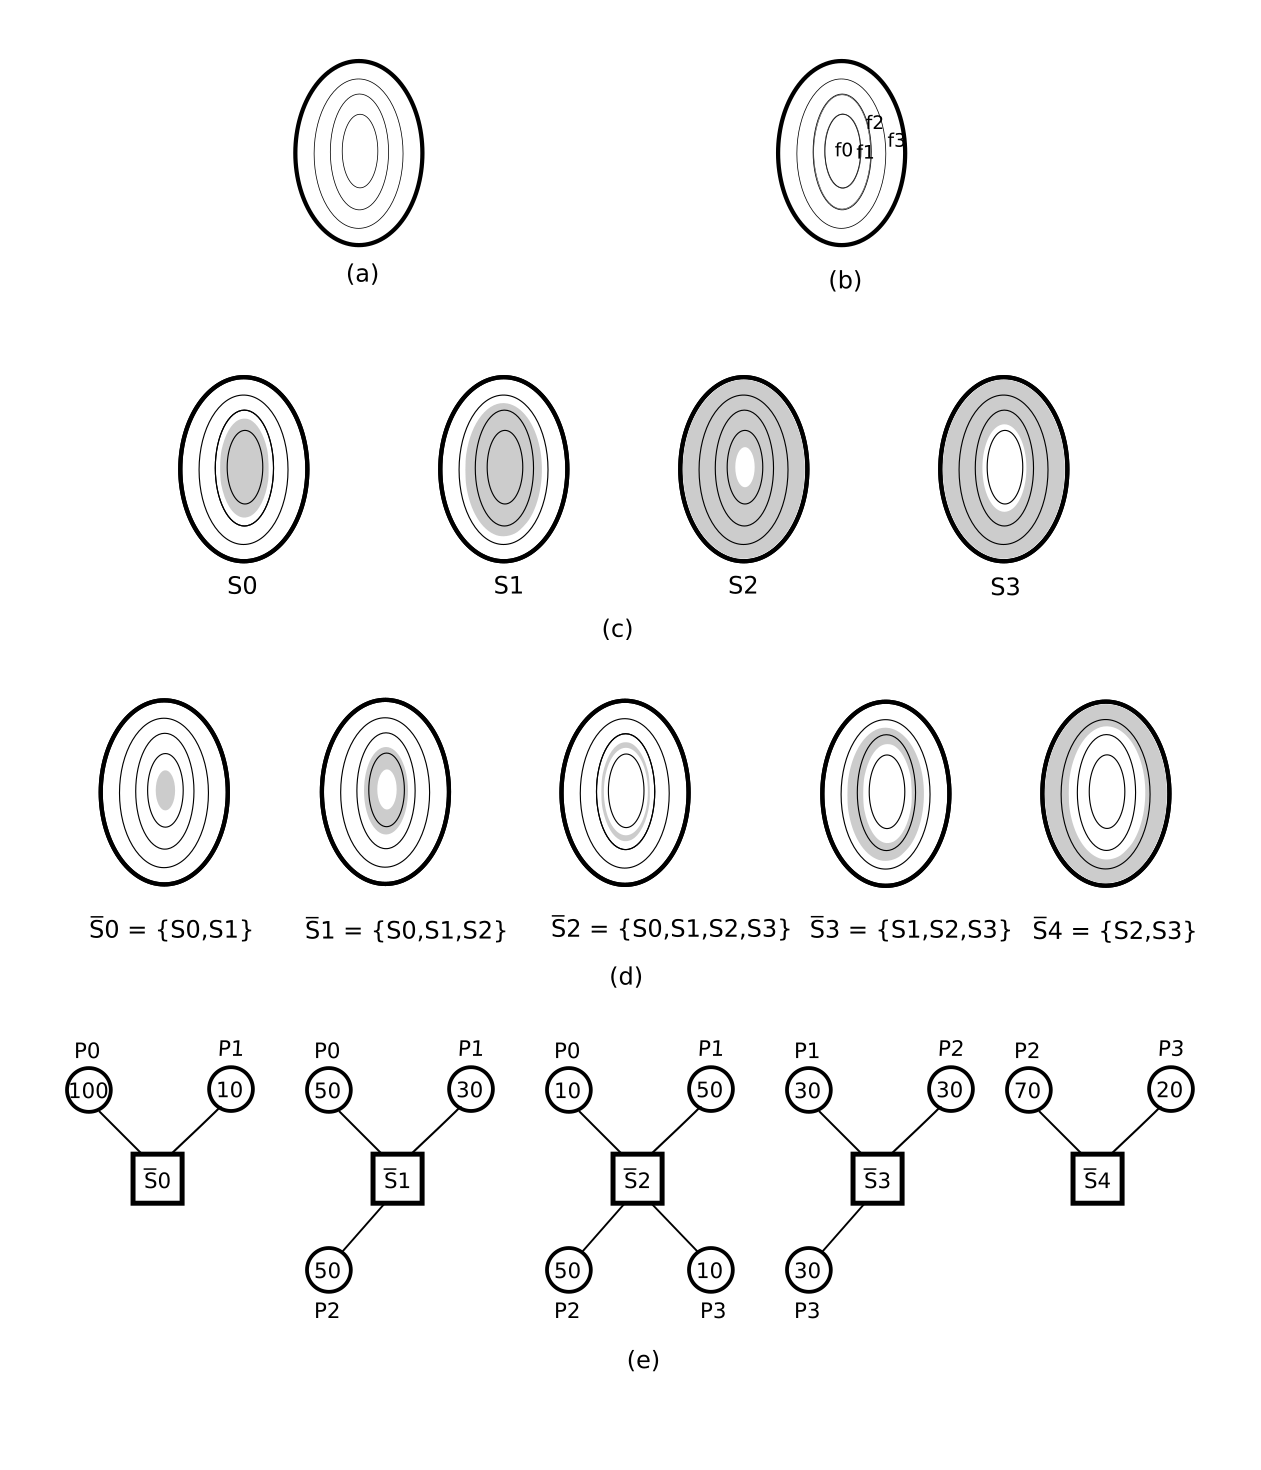
\includegraphics[width=.4\textwidth]{../figures/xgcm_ngraph_construction.png}
  \caption{An example of overlapping safe zones and the N-graph constructed from them.}
  \label{fig:sbars}
\end{figure}

In order to load balance this graph, we run diffusive techniques on the weights of the vertices
rather than the vertices. This means that instead of migrating graph vertices, we migrate the
weight of the vertices across hyperedges to reduce the imbalance of load in the graph.

\begin{itemize}
\item Add particle selection after engpar.
\item Add results of using engpar vs not using engpar
\item Add timing results compared to an iteration of XGCM.
\end{itemize}

\section{Computational Fluid Dynamics}

\begin{itemize}
\item Briefly discuss CFD (FUN3D/Phasta).
\item Discuss vertex-based partition vs. element-based partition.
\item Discuss how EnGPar/Ngraph can support both.
\item Discuss the current approach in FUN3D for partitioning and our ideas to improve it.
\item Mention the boundary stack and our approach to better represent it.
\end{itemize}

\section{Results}

\begin{itemize}
\item Compare parmetis graph partitions vs. Zoltan hypergraph partitions
\item Then compare how EnGPar can balance each.
\item Use FUN3D runs to compare how different metrics affect the runtime.
\end{itemize}


\section{Future Works}

\begin{itemize}
\item accelerators
\item Other ideas for load balancing vertex-based partitions?
\end{itemize}

{\color{red} Add bibliography stuff here}

\end{document}
